\documentclass{beamer}
\mode<presentation>
{\usetheme{default}
 \usecolortheme{default}
 \usefonttheme{default}
 \setbeamertemplate{navigation symbols}{}
 \setbeamertemplate{caption}[numbered]} 
\usepackage[english]{babel}
\usepackage[utf8]{inputenc}
\usepackage[T2A]{fontenc}
\usepackage{graphicx}
\usepackage{subcaption}
\usepackage{tikz}
\usepackage{amsmath,amssymb}
\usepackage{hyperref}
\hypersetup{colorlinks,linkcolor=,urlcolor=blue}
\newtheorem{Th}{Теорема}
\newcommand{\tr}{\mathrm{trace}}
\usefonttheme[onlymath]{serif}
\newcommand{\Q}{{\color{red}{\textbf{Q}}}}
\DeclareMathOperator*{\argmin}{\arg\min}
\DeclareMathOperator*{\argmax}{\arg\max}

\usepackage{caption}
\captionsetup[figure]{labelformat=empty}

\setbeamersize{text margin left=0.5cm,text margin right=1cm} 

\newcounter{saveenumi}
\newcommand{\seti}{\setcounter{saveenumi}{\value{enumi}}}
\newcommand{\conti}{\setcounter{enumi}{\value{saveenumi}}}

\resetcounteronoverlays{saveenumi}

%%%%%%%%%%%%%%%%%%%%%%%%%%%%%%%%%%%%%%%%%%%%%%
% Formatting for title page
\addtobeamertemplate{navigation symbols}{}{    \usebeamerfont{footline}%
    \insertframenumber \ /  \inserttotalframenumber }
    
    
\title[GD \& Co.]{Advanced optimization methods\\
Gradient descent and beyond. Part 1}
\author{Alexandr Katrutsa}
\institute{ 
MIPT department of applied mathematics and computer science\\
%\vspace{-0.5cm}
\begin{figure}
%\begin{subfigure}[c]{0.3\textwidth}
%\includegraphics[scale=0.3]{../pics/fivt_logo}
%\end{subfigure}
 
\includegraphics[scale=0.05]{../pics/fpmi_logo}
\end{figure}
%\vspace{-1cm}
}
\date{\today}
%%%%%%%%%%%%%%%%%%%%%%%%%%%%%%%%%%%%%%%%%%%%%%
\begin{document}
\begin{frame}
  \titlepage
\end{frame}

\begin{frame}{Plan for today}
\begin{itemize}
\item Gradient descent
\item Heavy-ball method
\item Nesterov accelerated GD
\item Why accelerated?
\end{itemize}
\end{frame}

\begin{frame}{Problem statement}
\[
\min_{x \in \mathbb{R}^n} f(x)
\]

\begin{itemize}
\item $f$ is smooth and convex
\item If $\mu \leq f''(x) \leq L, \; \mu \geq 0, \; L > 0$, then $f'$ is Lipschitz with constant $L$
\item If $\mu > 0$, then $f$ is $\mu$-strongly convex, and
\[
f(y) \geq f(x) + \langle f'(x), y - x \rangle + \frac{\mu}{2}\|y - x\|_2^2
\] 
\item Condition number $\kappa = \frac{L}{\mu}$
\end{itemize}
\end{frame}

\begin{frame}{Gradient descent}
\[
x_{k+1} = x_{k} - \alpha_k f'(x_k)
\]
\begin{itemize}
\item Explicit scheme for discretization of ODE
\[
\frac{dx}{dt} = -f'(x), \quad x(0) = x_0
\]
\item Minimization of upper bound at $x_k$
\[
\min_x f(x_k) + \langle f'(x_k), x - x_k \rangle + \frac{1}{2\alpha_k}\|x - x_k\|_2^2, 
\]
\item The best local descent direction
\[
f(x_k + h_k) \approx f(x_k) + \langle f'(x_k), h_k \rangle < f(x_k)
\]
\end{itemize}

\end{frame}

\begin{frame}{Step size selection}

\begin{itemize}
\item Constant $\alpha_k \equiv \mathrm{const} < \frac{2}{L}$
\item Decreasing sequence such that $\sum\limits_{k=1}^{\infty} \alpha_k = \infty$, i.e. $\frac{1}{k}, \frac{1}{\sqrt{k}}$, etc
\item Backtracking search: Armijo, Goldstein, Wolfe rules and others
\item Steepest descent: find the best possible $\alpha_k$
\end{itemize}

\begin{block}{Main point}
The best parameter you select gives you small gain in convergence! 
\end{block}

\end{frame}

\begin{frame}{Convergence: any $L$-smooth function}
\begin{equation*}
\begin{split}
f(x_{k+1}) &\leq f(x_k) + \langle f'(x_k), x_{k+1} - x_k \rangle + \frac{L}{2}\|x_{k+1} - x_k\|_2^2 = \\
& f(x_k) - \alpha_k \|f'(x_k)\|_2^2 + \frac{L \alpha^2_k}{2} \|f'(x_k)\|_2^2 = \\
& f(x_k) - \left(\alpha_k - \frac{L\alpha_k^2}{2}\right)\|f'(x_k)\|_2^2
\end{split}
\end{equation*}
\begin{itemize}
\item Descent condition: $\alpha_k - \frac{L\alpha_k^2}{2} > 0 \Rightarrow \alpha_k < \frac{2}{L}$
\item  The best $\alpha^*_k = \argmax\limits_{\alpha_k}\left(\alpha_k - \frac{L\alpha_k^2}{2}\right) = \frac{1}{L}$
\item $f(x_k) - f(x_{k+1}) \geq \frac{1}{2L}\|f'(x_k)\|_2^2$
\item $\frac{1}{2L} \sum\limits_{k=0}^T \|f'(x_k)\|_2^2 \leq f(x_0) - f(x_{T+1}) \leq f(x_0) - f^*$
\item $f$ is bounded below, $\|f'(x_k)\|_2 \to 0, \; k \to \infty$
\end{itemize}
\end{frame}

\begin{frame}{Convergence: $L$-smooth convex case}
\begin{block}{Theorem}
Let $f$ be $L$-smooth convex function and $\alpha = \frac{1}{L}$, then GD converges as
\[
f(x_{k+1}) - f^* \leq \frac{2L\|x - x_0\|^2_2}{k+4} = \mathcal{O}(1 / k)
\]
\end{block}
\end{frame}

\begin{frame}{Convergence: $\mu$-strongly convex case}
\begin{itemize}
\item $\mu$-strong convexity implication
\[
f(z) \geq f(x_k) + \langle f'(x_k), z - x_k \rangle + \frac{\mu}{2}\| z - x_k \|_2^2
\]
\item Minimize both side on $z$
\[
f(x^*) \geq f(x_k) - \frac{1}{2\mu} \|f'(x_k)\|_2^2, \quad \|f'(x_k)\|_2^2 \geq 2\mu (f(x_k) - f^*)
\]
\item Recall that for $\alpha_k \equiv \frac{1}{L}$
\[
f(x_{k+1}) \leq f(x_k) - \frac{1}{2L}\|f'(x_k)\|_2^2
\]
\item Finally get linear rate
\[
f(x_{k+1}) - f^* \leq \left( 1 - \frac{1}{\kappa}\right) (f(x_k) - f^*)
\]
\end{itemize}
\end{frame}

\begin{frame}{More precise estimate}
\begin{block}{Theorem}
Let $f$ be $L$-smooth and $\mu$-strongly convex and $\alpha_k = \frac{2}{\mu + L}$, then GD converges as
\[
f(x_k) - f^* \leq \frac{L}{2}\left( \frac{L - \mu}{L + \mu} \right)^{2k} \|x_0 - x^*\|^2_2
\]
\end{block}
\end{frame}

\begin{frame}{Gradient descent highlights}
\begin{itemize}
\item Easy to implement
\item It converges at least to stationary point
\item Recent paper\footnote{\url{https://arxiv.org/pdf/1602.04915.pdf}} shows that GD converges to a local minimizer \textbf{almost sure} with random initialization
\item Linear convergence in strongly convex case
\item It strongly depends on the condition number of $f''(x)$, random initial guess vector can help
\end{itemize}
\end{frame}

\begin{frame}{Heavy-ball method (Polyak, 1964)}
\[
x_{k+1} = x_k - \alpha_k f'(x_k) + {\color{red}{\beta_k(x_k - x_{k-1})}}
\]
\begin{figure}
\centering
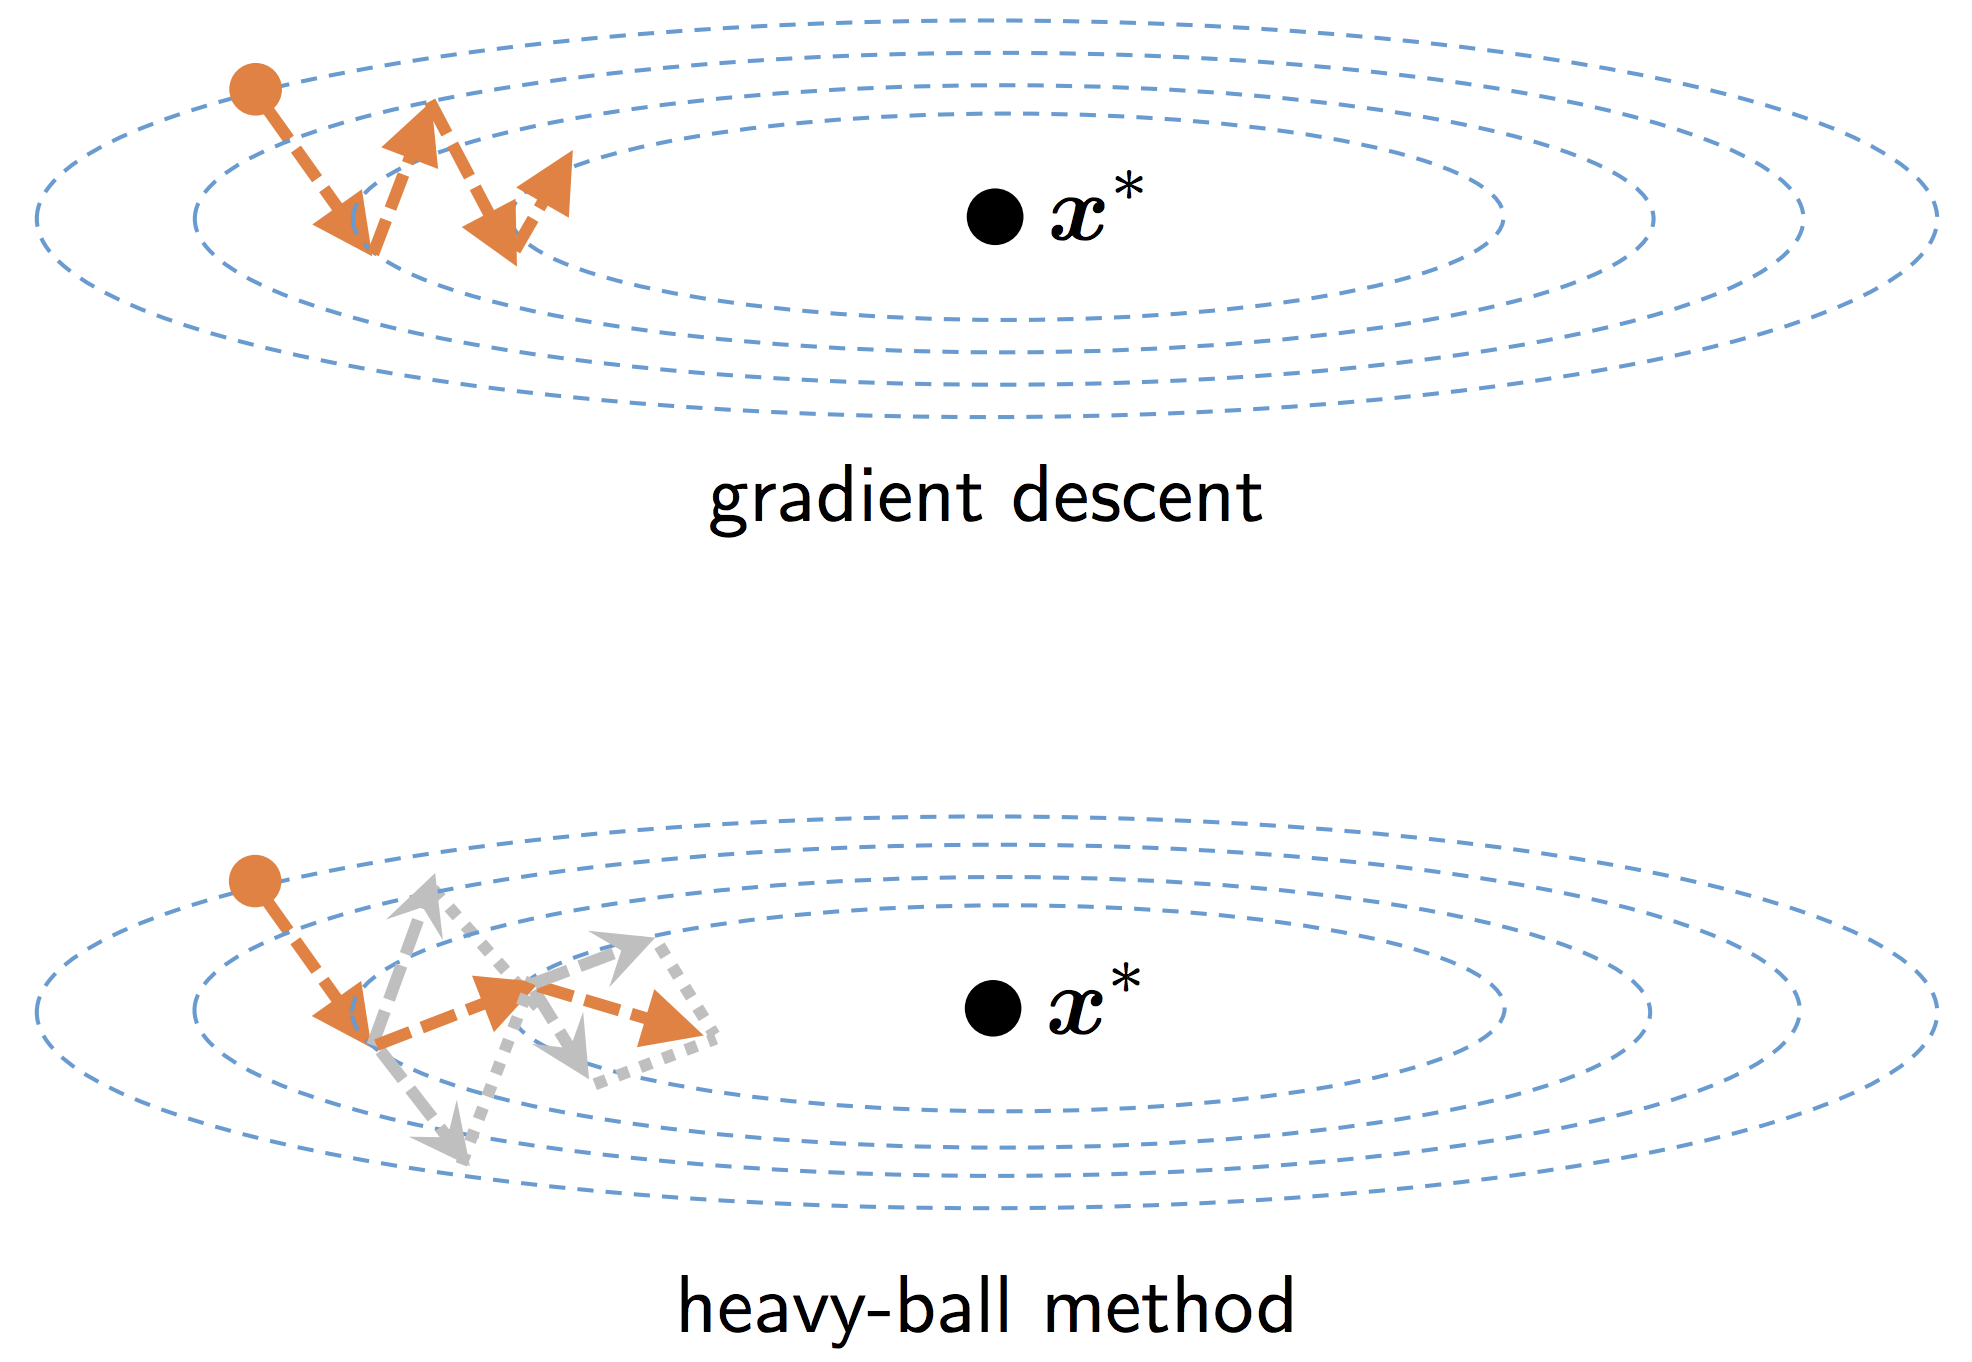
\includegraphics[scale=0.1]{heavy_ball.png}
\caption{Plot is from here\footnote{\url{http://www.princeton.edu/~yc5/ele538_optimization/lectures/accelerated_gradient.pdf}}}
\end{figure}

\begin{itemize}
\item Two-step non-monotone method
\item Discretization of the ODE with friction term
\[
\ddot x + b \dot x + a f'(x) = 0
\] 
\item Connection between ODE and optimization methods
\item CG is special case of this form
\end{itemize}

\end{frame}

\begin{frame}{Convergence: $\mu$-strongly convex}
\begin{itemize}
\item Rewrite method as 
\begin{equation*}
\begin{split}
\begin{bmatrix}
x_{k+1}\\
x_k
\end{bmatrix}
 = 
 \begin{bmatrix}
 (1 + \beta_k)I & -\beta_k I\\
 I & 0
 \end{bmatrix}
 \begin{bmatrix}
 x_k\\
 x_{k-1}
 \end{bmatrix}
 +
 \begin{bmatrix}
 -\alpha_k f'(x_k)\\
 0
 \end{bmatrix}
\end{split}
\end{equation*}
\item Use theorem from calculus
\begin{equation*}
\begin{split}
\begin{bmatrix}
x_{k+1} - x^*\\
x_k - x^*
\end{bmatrix}
 = 
 \underbrace{
 \begin{bmatrix}
 (1 + \beta_k)I - \alpha_k \int_0^1 f''(x(\tau))d\tau & -\beta_k I\\
 I & 0
 \end{bmatrix}
 }_{=A_t}
 \begin{bmatrix}
 x_k - x^*\\
 x_{k-1} - x^*
 \end{bmatrix},
\end{split}
\end{equation*}
where $x(\tau) = x_k + \tau(x^* - x_k) $
\item Convergence depends on the spectrum of the iteration matrix $A_t$
\item Select $\alpha_k$ and $\beta_k$ to make spectral radius the smallest 
\end{itemize}
\end{frame}

\begin{frame}{Parameter selection}
\begin{block}{Theorem}
Let $f$ be $L$-smooth and $\mu$-strongly convex. Then $\alpha_k = \frac{4}{(\sqrt{L} + \sqrt{\mu})^2}$ and $\beta_k = \max(|1 - \sqrt{\alpha_k L}|, |1 - \sqrt{\alpha_k \mu}|)^2$ gives
\begin{equation*}
\left \|
\begin{bmatrix}
x_{k+1} - x^*\\
x_k - x^*
\end{bmatrix}
\right \|_2
\leq \left( \frac{\sqrt{\kappa} - 1}{\sqrt{\kappa} + 1} \right)^k
\left \|
\begin{bmatrix}
x_1 - x^*\\
x_0 - x^*
\end{bmatrix}
\right \|_2
\end{equation*}
\end{block}
\begin{itemize}
\item Parameters depend on $L$ and $\mu$
\item Faster than GD
\item Similar to CG for $\mu$-strongly convex quadratic
\item Can such estimate be extend to $L$-smooth convex function?
\end{itemize}
\end{frame}

\begin{frame}{Heavy-ball method highlights}
\begin{itemize}
\item Simple two-step method
\item Converges much faster than GD with appropriate $\alpha_k$, $\beta_k$
\item CG is particular case
\item Proof only for $\mu$-strongly convex functions
\end{itemize}
\end{frame}

\begin{frame}{Nesterov accelerated GD (Nesterov, 1983)}
One of possible notation variant
\begin{equation*}
\begin{split}
& y_0 = x_0 \\
& x_{k+1} = y_k - \alpha_k f'(y_k)\\
& y_{k+1} = x_{k+1} + \frac{k}{k + 3} (x_{k+1} - x_k)
\end{split}
\end{equation*}

\begin{itemize}
\item Heavy-ball comparison
\item ODE interpretation again
\item Non-monotone, too
\item More details and options see in Part 2
\end{itemize}
\end{frame}

\begin{frame}{Nesterov method visualization}

\begin{figure}
\centering
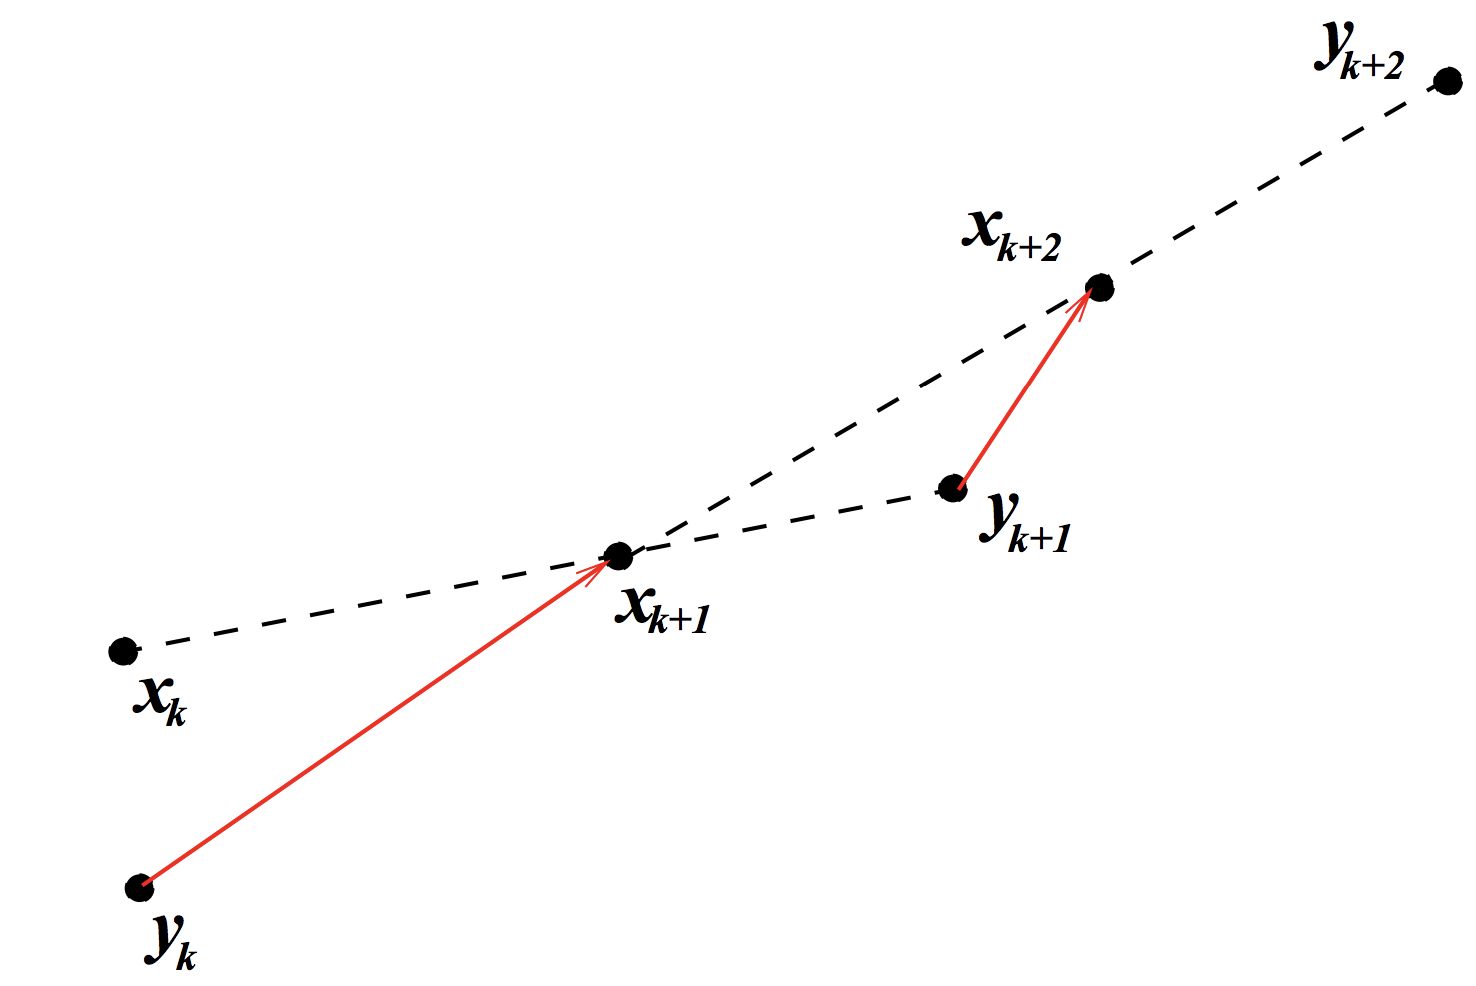
\includegraphics[scale=0.3]{nesterov_plot}
\end{figure}



\end{frame}

\begin{frame}{Convergence: $L$-smooth convex}
\begin{block}{Theorem}
Let $f$ be convex and $L$-smooth. Assume $\alpha_k = \frac{1}{L}$. Then Nesterov method converges as
\[
f(x_k) - f^* \leq \frac{2L \|x_0 - x^*\|_2^2}{(k+1)^2} = \mathcal{O}(1/k^2)
\]
\end{block}
\begin{itemize}
\item Compare with GD convergence
\item Iteration cost is almost the same
\end{itemize}
\end{frame}

\begin{frame}{Convergence: $\mu$-strongly convex}
\begin{block}{Theorem}
Nesterov method for $\mu$-strongly convex function $f$ (with some additional assumptions) converges as 
\[
f(x_k) - f^* \leq L\|x_k - x_0\|_2^2 \left(1 - \frac{1}{\sqrt{\kappa}} \right)^k
\]
\end{block}

\begin{itemize}
\item Faster than GD
\item Similar to heavy-ball method
\end{itemize}
\end{frame}

\begin{frame}{Practical issues}
\begin{itemize}
\item Rippling behaviour and restarts
\[
f(x_1, x_2) = 2 \cdot 10^{-2}x_1^2 + 5 \cdot 10^{-3}x^2_2 \to \min, \; x_0 = (1, 1)
\]
\begin{figure}
\centering
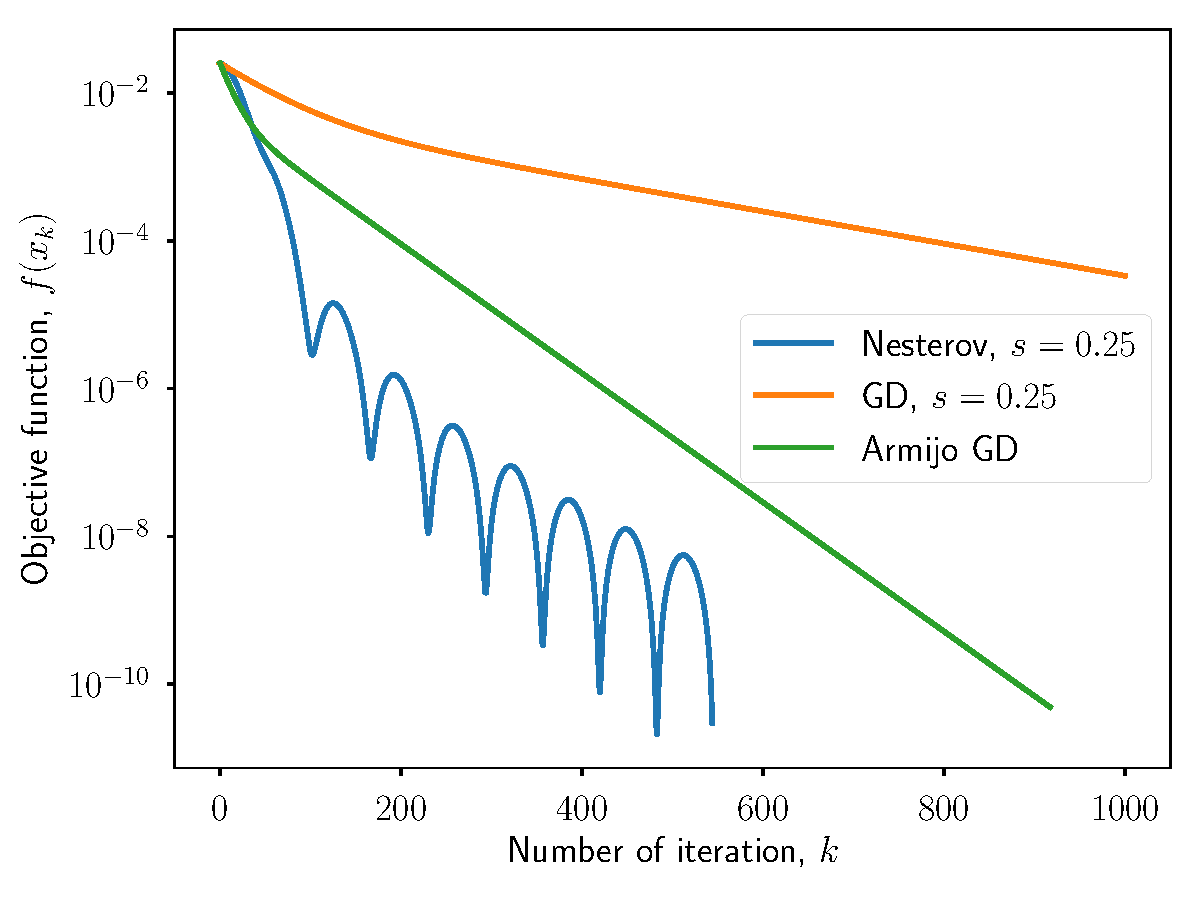
\includegraphics[scale=0.4]{nesterov_gd}
\end{figure}
\item Estimate of $\mu$ and $L$ is separate problem
\end{itemize}
\end{frame}

\begin{frame}{Why acceleration?}
\begin{itemize}
\item It is faster than GD
\item Is there even faster FOM for considered problems?
\end{itemize}
\end{frame}

\begin{frame}{Lower bound concept}
If we have access only to (sub)gradient in any point:
 
\begin{table}
\centering
\begin{tabular}{|c|c|}
\hline
Convex functions & Lower bound\\
\hline
Nonsmooth & $f(x_k) - f^* \geq \frac{G\|x^* - x_0\|_2^2}{2(1 + \sqrt{k+1})}$\\
\hline
$L$-smooth convex & $f(x_k) - f^* \geq \frac{3L \|x_0 - x^*\|_2^2}{32(k+1)^2}$\\
\hline
$\mu$-strongly convex & $f(x_k) - f^* \geq \frac{\mu}{2}\left(\frac{\sqrt{\kappa} - 1}{\sqrt{\kappa} + 1} \right)^{2k} \|x_0 - x^*\|_2^2$\\
\hline
\end{tabular}
\end{table}
\end{frame}

\begin{frame}{To be discussed in part 2}
\begin{itemize}
\item Proximal methods
\item Mirror descent
\end{itemize}
\end{frame}

\begin{frame}{Next class announce}
Some proofs from this class.

Stochastic modifications of the considered methods today
\begin{itemize}
\item SAG
\item SAGA
\item SVRG
\item SEGA
\item ...
\end{itemize}
\end{frame}

\begin{frame}[allowframebreaks]{References}

\nocite{nesterov1983method}\nocite{beck2017first}
\nocite{polyak1964some} \nocite{o2015adaptive}\nocite{nemirovsky1983problem} \nocite{su2014differential}
\bibliographystyle{apalike}
\bibliography{lib}
% \url{https://epubs.siam.org/doi/book/10.1137/1.9781611974997 }
\end{frame}

\end{document}